% Drop-in replacement for the exploratory attention appendix.
% Requires graphicx; compile from paper/ with the supplied figures/ directory.
\section{Exploratory attention inspection}
\label{appendix:attention}

We inspect attention as a descriptive diagnostic across ordered compliance (OC),
key-inversion parity (KIP), and CKD$\to$ESRD prediction. Attention allocation does
not establish the causal contribution of a head or identify a unique internal
algorithm. Our mechanism claims therefore rely on the feature-space and input
audits, with attention providing complementary observations.

\paragraph{OC: models and measurement.}
We analyze BERT-base and RoBERTa-base with full fine-tuning,
Llama-3.1-8B with LoRA, and Qwen3.8-27B with QLoRA on OC-Deterministic,
plus a separate Qwen3.8-27B QLoRA fit on OC-Noisy. Each task-specific fit starts
from the pretrained base, without KIP fine-tuning. The encoders and Llama use
the same 200K training subset; Qwen uses 400K. Both Qwen fits were capped at
six completed epochs, with validation loss selecting epoch 5 for deterministic
OC and epoch 6 for noisy OC.

All five audits use the same 1,000 held-out sequences, sampled proportionally
by the latent clean label (seed 9950): 292 compliant and 708 non-compliant. The corrected
OC rule uses key letters $\{W,D,Q,J,X,U\}$ and lag $\lambda=7$.
For each key-source event, we measure attention to key events at distance
$\lambda$, other key events, and non-key events. Lag membership is positional;
it does not require that the pair satisfy the secret rank ordering. Self-attention
and prompt/special-token attention are recorded separately. Target-token masses
are summed within events and query tokens are averaged within source events.
We respect each model's visibility mask: bidirectional for encoders and causal
for decoders.

For each example, layer, and head, we divide the mean attention mass for an
eligible target category by its expected mass under uniform attention over
visible tokens. We then average these ratios over eligible examples and heads.
Thus enrichment above one denotes allocation above that visibility-matched
baseline. Queries without visible targets in a category are omitted; the lag
category has support in 465 of the 1,000 sequences. Categories consequently
have different eligibility sets and their averaged curves are not an additive
partition. Primary summaries include both outcomes, without selecting examples
by prediction correctness. For hybrid Qwen3.8-27B, we inspect only its 16 standard
attention blocks; recurrent blocks are excluded.

\paragraph{OC: localized lag enrichment and input controls.}
Figure~\ref{fig:attn_layer_summary} shows localized enrichment for lag-connected
keys. Using one-based physical layer numbers, head-averaged lag enrichment peaks
at 3.18 in BERT layer 7, 1.42 in RoBERTa layer 12, and 2.24 in Llama layer 12.
Both Qwen fits peak at physical layer 28: 6.16 for deterministic OC and 4.18 for
noisy OC. These are descriptive maxima. Enrichment varies across depth and heads;
it is not a consistently elevated signal throughout the network. Normalization
accounts for target availability, but does not control differences in architecture,
tokenization, training size, or adaptation method.

We additionally perturb the same 200 fixed sequences while preserving letter
counts. Oracle-verified label-changing permutations were found for 192 sequences
within 64 proposals each. All four deterministic-OC models correctly change their
predictions on all 192 permutations and preserve their predictions on all 200
distractor-only swaps. Noisy Qwen correctly follows 187 of the 192 label changes
and likewise has no prediction flips on distractor swaps. These diagnostics use
threshold 0.5 and latent clean labels, including for noisy OC. The conditional
192-example subset is not an unbiased performance estimate. The controls establish
sensitivity to order beyond letter counts on the tested inputs; they do not
establish the causal necessity of the displayed attention patterns. All four
deterministic fits classify the 1,000 sampled sequences correctly at this threshold,
so these audits provide no missed-compliant group for a correctness comparison.

\begin{figure}[t]
\centering
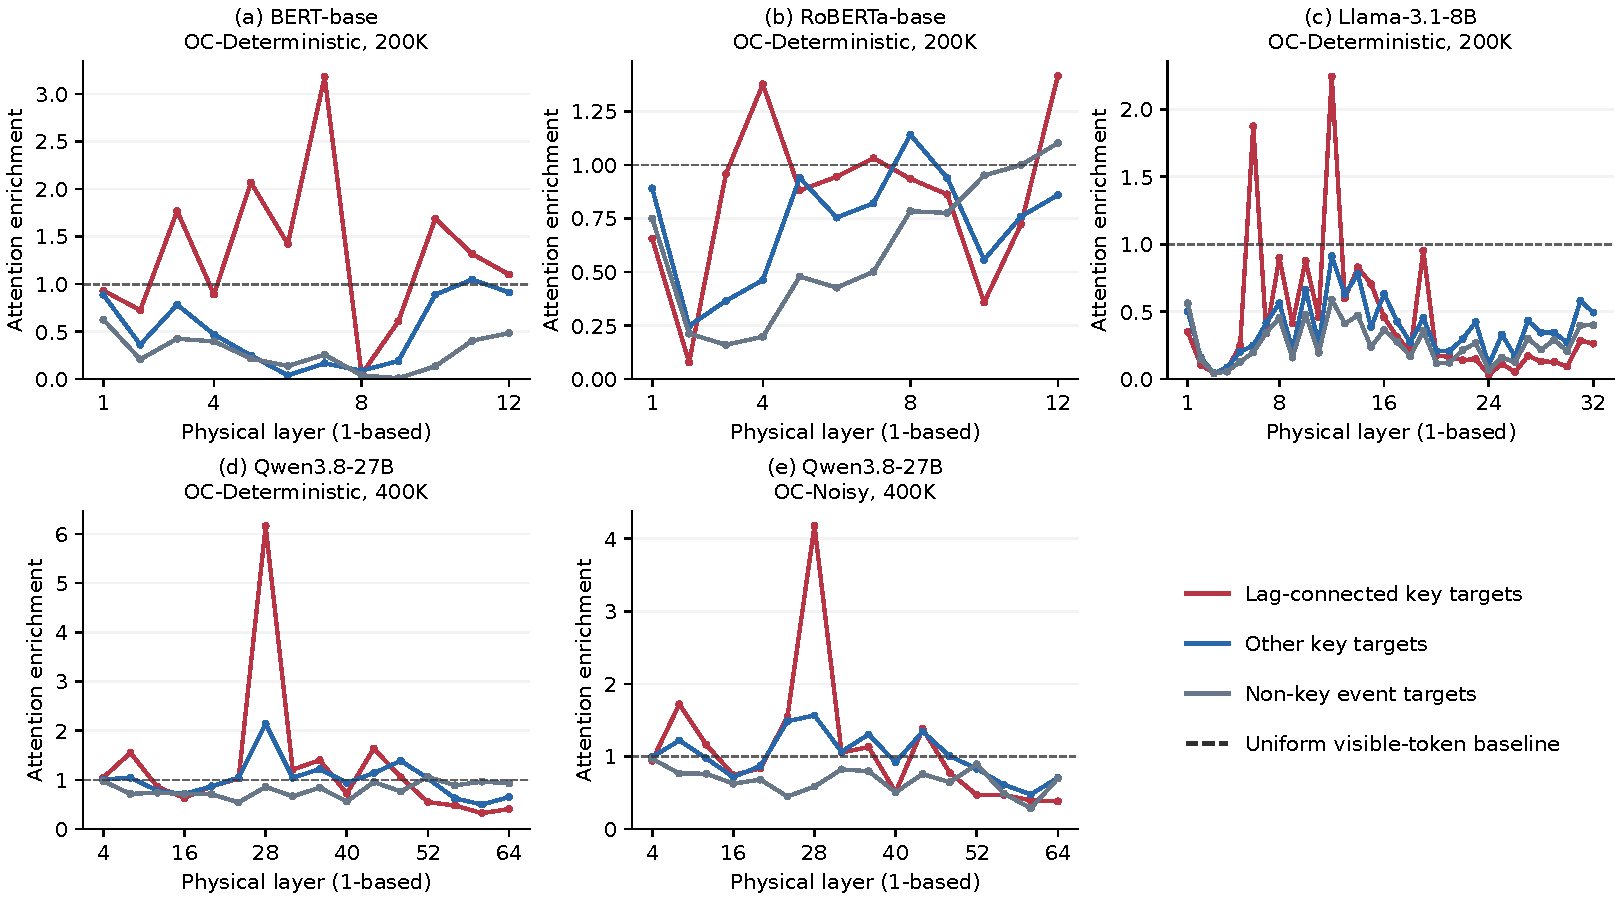
\includegraphics[width=\textwidth]{figures/attention_oc_profiles_20260925.pdf}
\caption{OC attention enrichment across physical layers for the five completed
audits. Red: lag-connected key targets; blue: other key targets; gray: non-key
event targets. Dashed lines indicate uniform attention over visible tokens.
Curves average per-example enrichment over eligible examples and heads, using
all sampled outcomes. Target categories have different eligibility sets.
Layer numbering is one-based and panels use separate $y$-axis ranges.
Qwen panels include standard attention blocks only. Localized lag enrichment is
visible, but the profiles are descriptive and do not constitute a controlled
architecture comparison or a causal attribution.}
\label{fig:attn_layer_summary}
\end{figure}

\paragraph{KIP: key-order sensitivity without a unique attention signature.}
We inspect 22 saved checkpoints on 1,000 fixed held-out examples per task:
BERT-base and RoBERTa-base with full fine-tuning and LoRA on M4/M6;
Llama-3.2-1B with full fine-tuning on M4/M6; and Llama-3.1-8B LoRA,
Qwen2.5-14B QLoRA, and Qwen3.8-27B QLoRA on M4 at 4K, 40K, 120K, and
200K training examples. Measurements distinguish key, inversion/non-inversion,
distractor, self, and readout attention using visibility-matched baselines.
The four successful M4 checkpoints---Llama-3.2-1B and the three larger decoders
at 200K---have test AUROC 1.0 and flip their predictions on all 200 tested
key transpositions, with no flips on 200 distractor transpositions.
Their attention profiles show model-dependent key routing rather than a common
preference for inversion pairs. Key-preferring heads also occur in chance-level
checkpoints. Attention to relevant symbols therefore does not by itself establish
the computation of inversion parity.
Figure~\ref{fig:attn_kip_summary} shows the four successful M4 checkpoints;
this is a descriptive selection from the 22 audited checkpoints.

\begin{figure}[t]
\centering
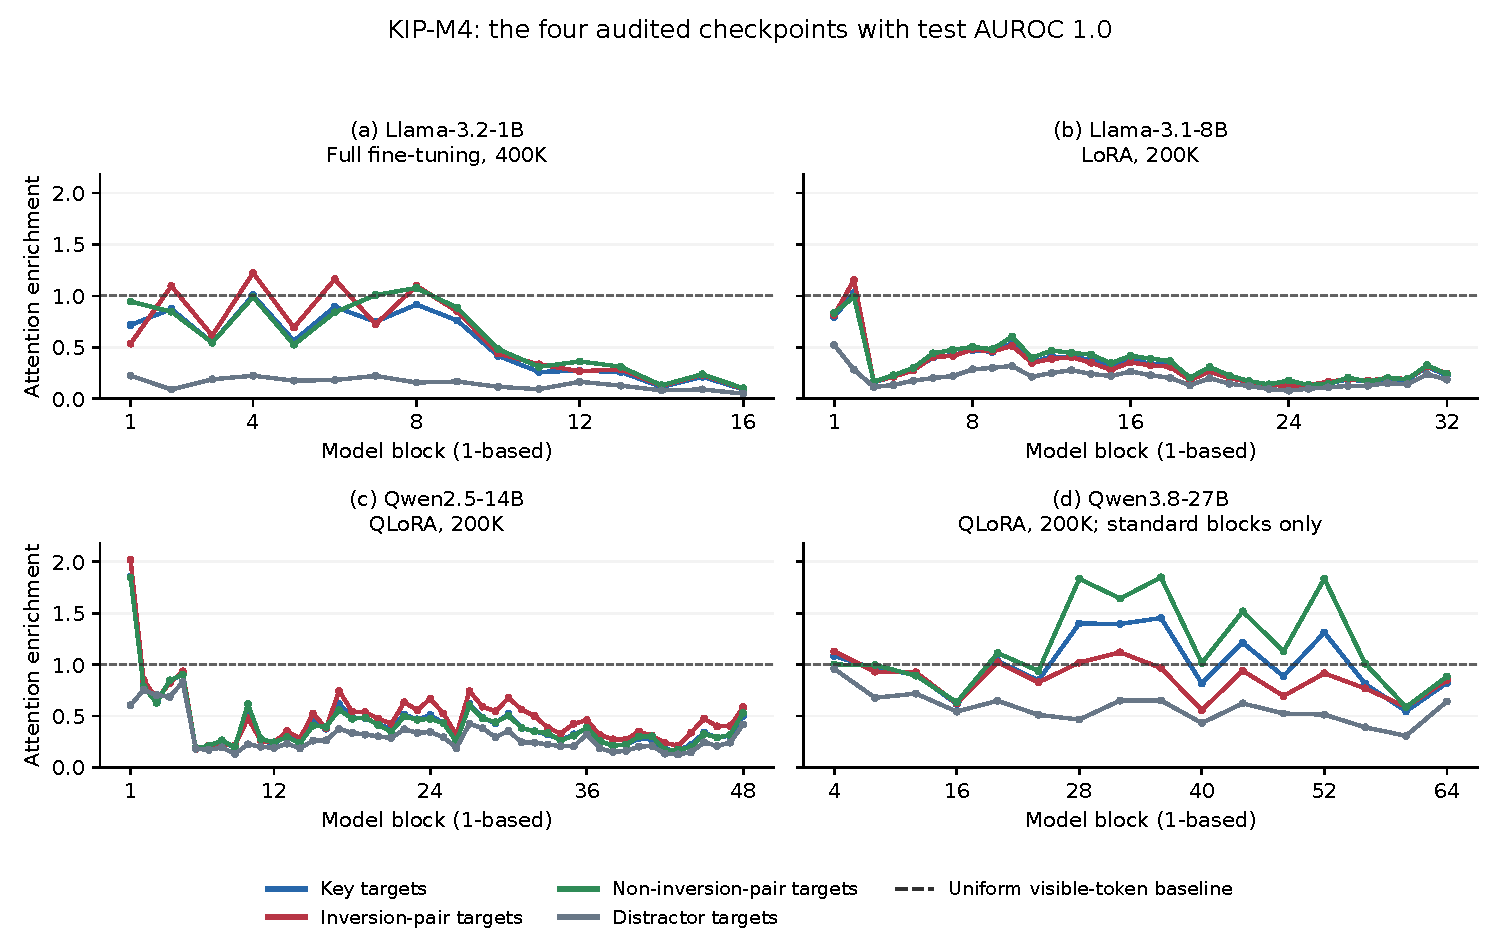
\includegraphics[width=\textwidth]{figures/attention_kip_m4_profiles_20260925.pdf}
\caption{Attention enrichment for the four audited KIP-M4 checkpoints with
test AUROC 1.0. Llama-3.2-1B uses full fine-tuning on 400K examples; the larger
decoders use LoRA or QLoRA on 200K. Blue: key targets excluding the source
event; red: inversion-pair targets; green: non-inversion-pair targets; gray:
distractors. Dashed lines denote uniform attention over all visible tokens,
including self and prompt/special tokens. Curves average per-example
mass-to-baseline ratios over eligible examples and then heads. Key and distractor
curves use all 1,000 sampled examples; inversion and non-inversion curves use
971 and 961 eligible examples, respectively. Categories overlap and conditional
averaging differs, so the curves are not additive. Model-block indices are
one-based. Only standard attention blocks are shown for Qwen3.8-27B; connecting
lines do not measure its intervening recurrent blocks. These selected-checkpoint
profiles describe model-dependent routing and do not identify an internal
parity algorithm or provide a controlled architecture comparison.}
\label{fig:attn_kip_summary}
\end{figure}

\paragraph{MIMIC-IV CKD: paired readout attention.}
For BERT-base, RoBERTa-base, Llama-3.1-8B, and Qwen3.8-27B, we compare
separately trained ordered and shuffled models on the same 1,000 held-out
patients, including 77 progressors. We inspect the classifier readout query
(CLS for encoders, the last unmasked token for decoders); Qwen again contributes
only its 16 standard attention blocks. We aggregate repeated CCS-code occurrences,
average code masses over heads and audited layers, then normalize within each
patient to sum to one over CCS codes, excluding prompt mass.
The mean paired overlap, defined as one minus total-variation distance
between these code distributions, is 0.850 for BERT, 0.848 for RoBERTa, 0.703
for Llama, and 0.674 for Qwen. This describes shared allocation to clinical
content, without identifying causal risk factors or proving order invariance.
The comparison changes both model weights and input order. Moreover, encoders
truncate at 512 tokens, affecting 191 BERT and 188 RoBERTa sampled patients,
whereas both decoders retain full histories. Shuffling can change which events
remain visible after truncation, precluding an equal-context architecture comparison.
Figure~\ref{fig:attn_ckd_summary} visualizes the layer-wise allocation to diagnosis
events and the dispersion of readout attention for both conditions.

\begin{figure}[t]
\centering
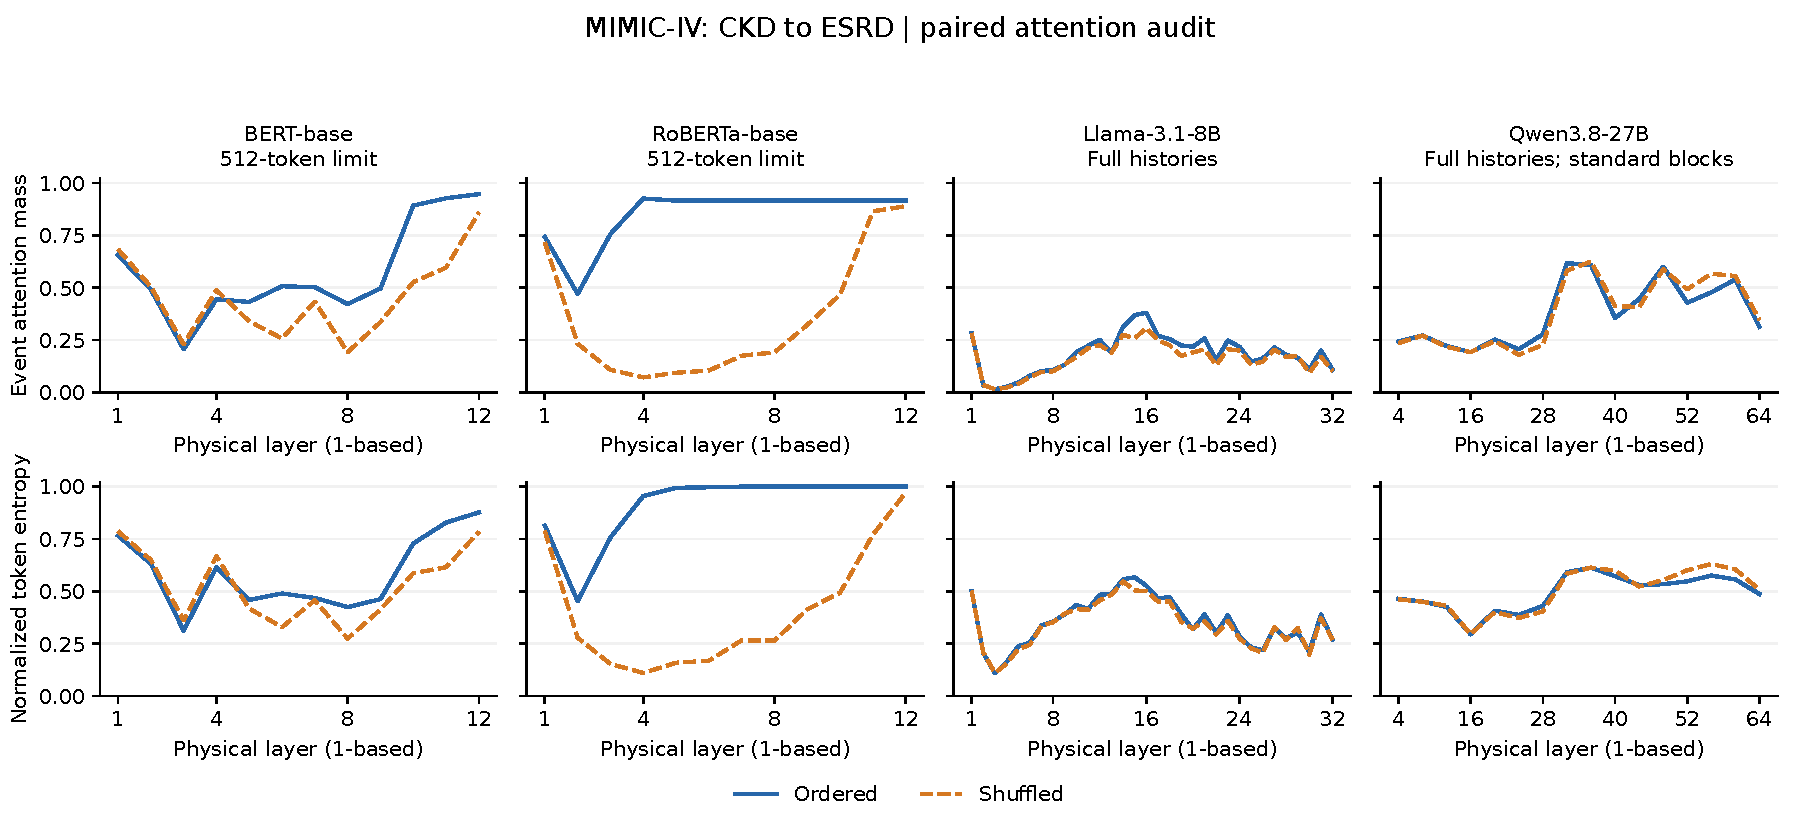
\includegraphics[width=\textwidth]{figures/attention_ckd_profiles_20260925.pdf}
\caption{MIMIC-IV CKD$\to$ESRD readout attention in separately trained ordered
(solid blue) and shuffled (dashed orange) models on the same 1,000 held-out
patients. Top: attention mass assigned to complete visible diagnosis events.
Bottom: token-attention entropy normalized by the logarithm of the visible token
count; higher values indicate more diffuse allocation. Both quantities are
averaged over heads within each patient and then over patients at each physical
layer. Encoders use the CLS query and a 512-token window; decoders use the last
unmasked query and full histories. Qwen includes only its 16 standard attention
blocks. Layers are numbered from one. Conditions differ in model weights and
input order, and encoder truncation can change visible content. The profiles
are descriptive, not a controlled comparison of architectures or causal effects
of shuffling.}
\label{fig:attn_ckd_summary}
\end{figure}

\paragraph{Fidelity and limits.}
OC and CKD diagnostics preserve the native forward computation and reproduce
saved test probabilities with maximum absolute error below $3\times10^{-8}$.
KIP includes six retained earlier eager-attention audits and sixteen native-attention
audits; all satisfy the prespecified 0.02 reproduction tolerance, with maximum
observed error 0.015624. These are single-checkpoint diagnostics for each setting.
Neither attention allocation nor input perturbations isolate an internal causal
pathway. Establishing one would require interventions on heads, value pathways,
MLPs, or the classifier readout.
